\chapter{Análise Teórica}

A fundamentação analítica desta prática repousa sobre a modelagem de circuitos de primeira ordem no domínio da frequência complexa $s$, utilizando a Transformada de Laplace. O comportamento do filtro passa-baixa foi estudado sob três perspectivas distintas: na sua forma passiva isolada, acoplado a uma carga resistiva direta (evidenciando o efeito de carga) e, finalmente, isolado da carga através de um amplificador operacional configurado como \textit{buffer} \cite{4a_pratica.pdf}.

Para garantir a precisão e automatizar a manipulação algébrica das equações nodais, empregou-se o ambiente de computação simbólica Maxima. A partir das funções de transferência $H(s)$ deduzidas, extraíram-se os parâmetros críticos de operação: o ganho de tensão em corrente contínua (ganho DC) e a frequência de corte ($f_c$).

\section{Circuito 1: Filtro RC Passa-Baixa sem Carga}

A topologia base consiste num simples divisor de tensão formado por um resistor $R$ e um capacitor $C$. A tensão de saída $V_o(s)$ é tomada diretamente sobre os terminais do elemento capacitivo. 

\begin{figure}[H]
	\centering
	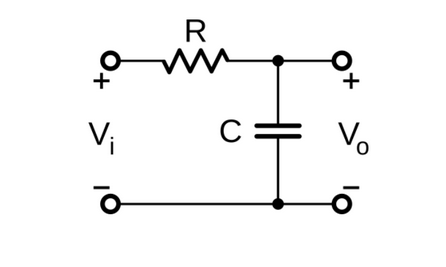
\includegraphics[width=0.6\textwidth]{FIGURAS/esquematico_circuito_1.png}
	\caption{Esquemático do filtro RC passa-baixa isolado (Circuito 1).}
	\label{fig:esquematico_c1}
\end{figure}

Substituindo os componentes pelas suas impedâncias no domínio de Laplace ($Z_R = R$ e $Z_C = \frac{1}{sC}$), a equação do divisor de tensão que rege o circuito estabelece que a função de transferência $H_1(s) = \frac{V_o(s)}{V_i(s)}$ é dada por:

\begin{equation}
	H_1(s) = \frac{Z_C}{Z_R + Z_C} = \frac{\frac{1}{sC}}{R + \frac{1}{sC}}
\end{equation}

Multiplicando o numerador e o denominador por $sC$, o Maxima simplifica a expressão teórica para o formato padrão:

\begin{equation}
	H_1(s) = \frac{1}{RCs + 1}
	\label{eq:h1}
\end{equation}

\subsection{Dedução Algébrica (Rascunhos)}

As Figuras \ref{fig:rascunho_c1_1} e \ref{fig:rascunho_c1_2} evidenciam o desenvolvimento matemático manuscrito das malhas e nós do Circuito 1, comprovando a obtenção da Equação \ref{eq:h1}.

\begin{figure}[H]
	\centering
	\begin{minipage}{0.45\textwidth}
		\centering
		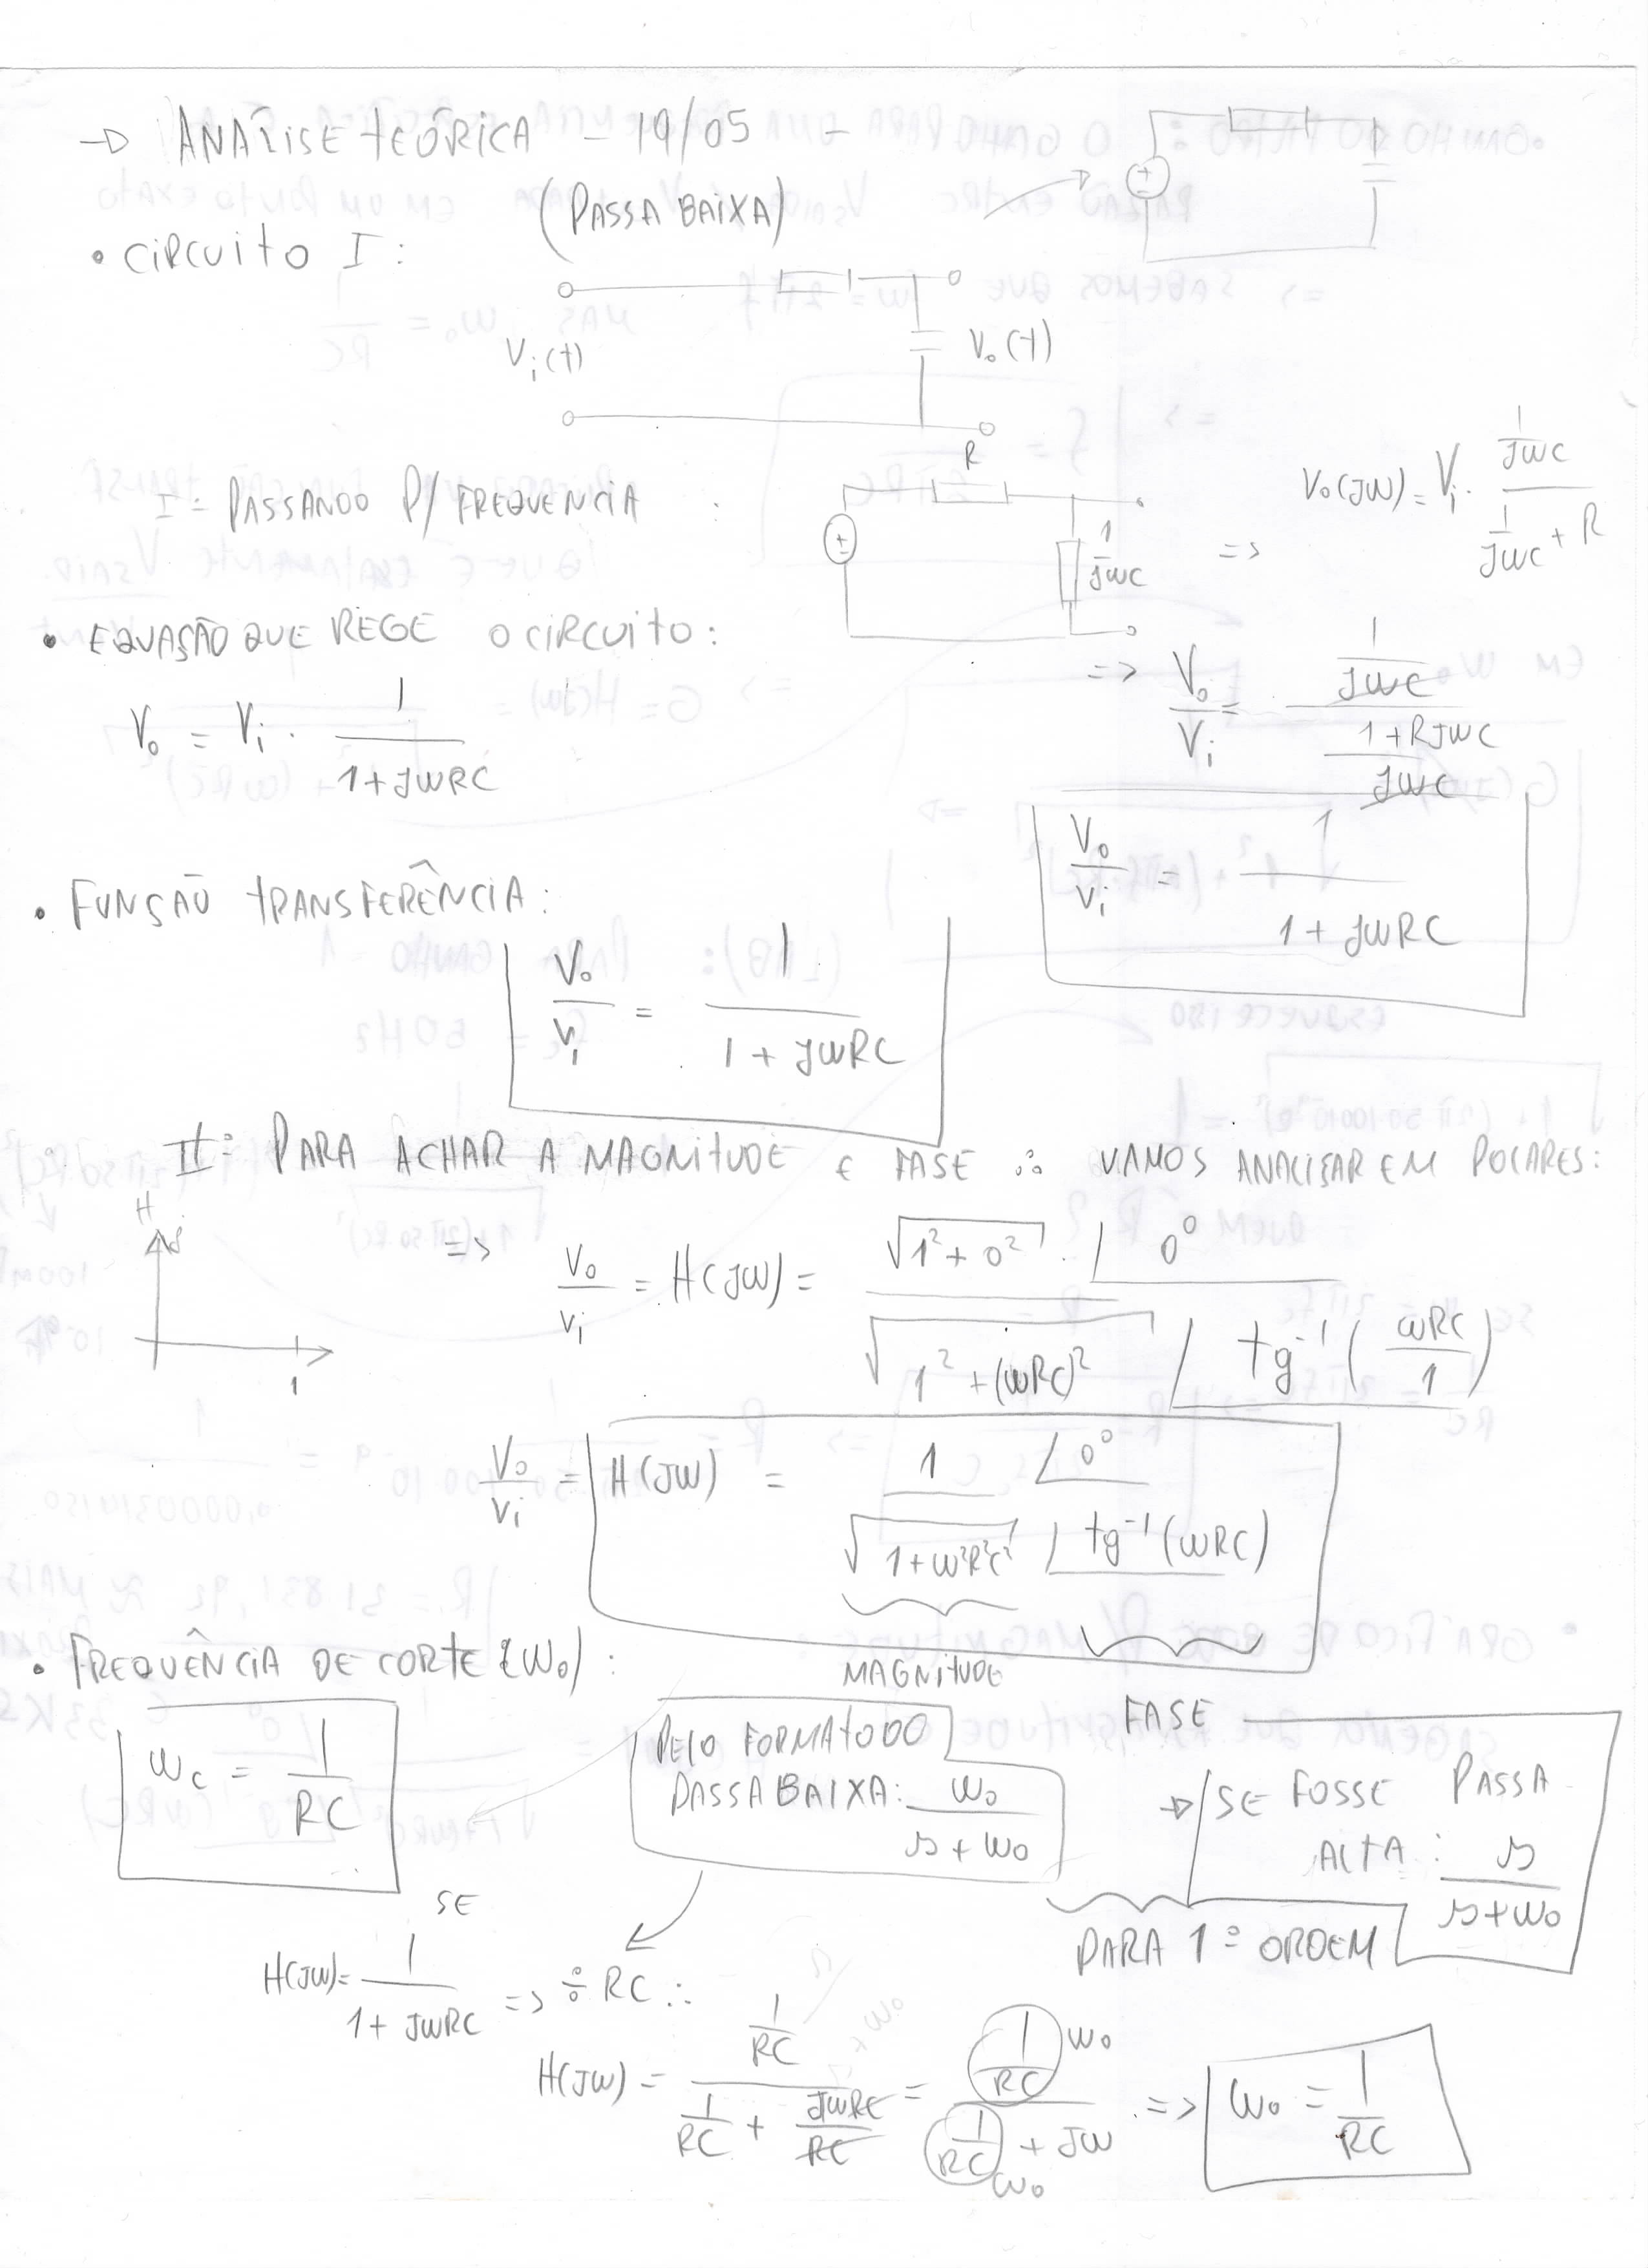
\includegraphics[width=\textwidth]{FIGURAS/rascunho_circuito_1_1.png}
		\caption{Modelagem inicial das impedâncias no domínio $s$ (Circuito 1).}
		\label{fig:rascunho_c1_1}
	\end{minipage}\hfill
	\begin{minipage}{0.45\textwidth}
		\centering
		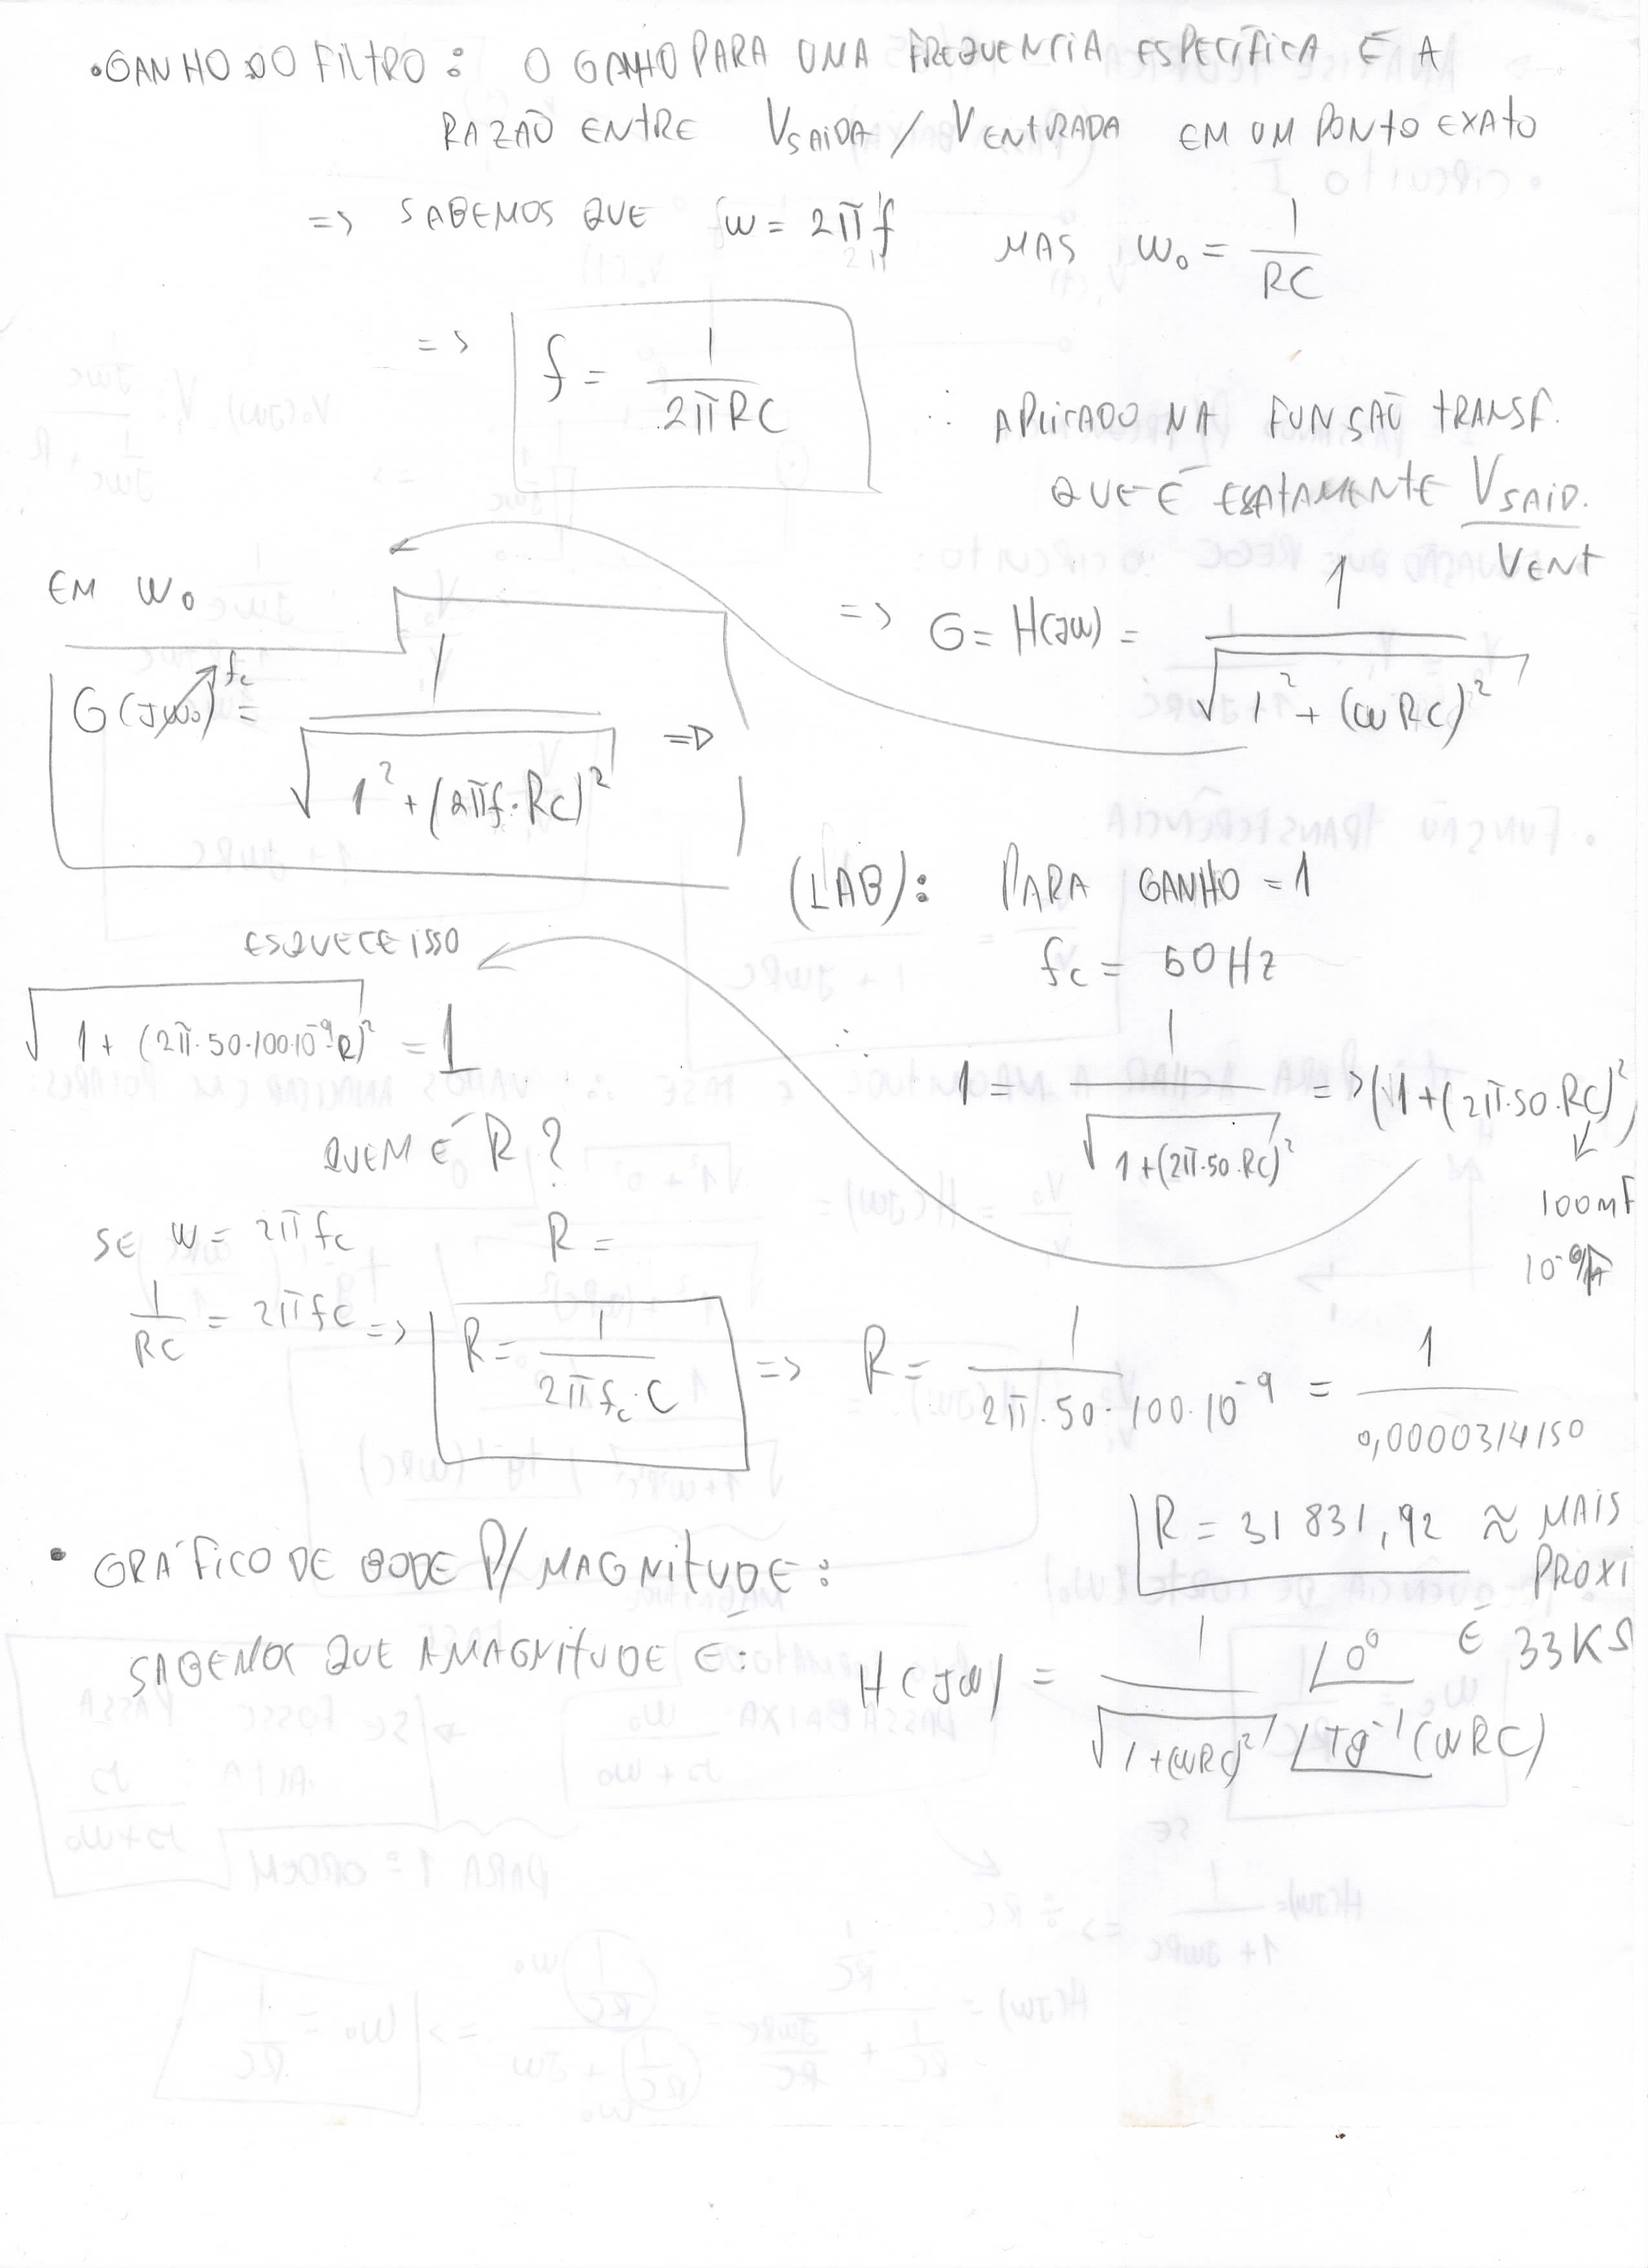
\includegraphics[width=\textwidth]{FIGURAS/rascunho_circuito_1_2.png} 
		\caption{Resolução e simplificação para $H_1(s)$.}
		\label{fig:rascunho_c1_2}
	\end{minipage}
\end{figure}

\subsection{Projeto do Filtro e Frequência de Corte}

Avaliando a Equação \ref{eq:h1} em frequências nulas ($s = 0$), o ganho estático teórico calculado é unitário ($1\text{ V/V}$ ou $0\text{ dB}$). A frequência de corte angular ($\omega_c$) ocorre quando o termo $RC\omega = 1$, o que define a frequência de corte em Hertz como $f_c = \frac{1}{2\pi R C}$.

O roteiro estipulou o projeto do filtro para uma frequência de corte $f_c = 50\text{ Hz}$ utilizando um capacitor fixo de $100\text{ nF}$. Resolvendo algebricamente para a resistência:

\begin{equation}
	R = \frac{1}{2\pi \cdot f_c \cdot C} = \frac{1}{2\pi \cdot 50 \cdot 100 \times 10^{-9}} \approx 31.831\text{ }\Omega
\end{equation}

Para a montagem em bancada, selecionou-se o valor comercial da série E24 mais próximo disponível no laboratório: $R = 33\text{ k}\Omega$. Recalculando a frequência de corte real com este componente comercial, o Maxima estimou o novo ponto de $-3\text{ dB}$ em:

\begin{equation}
	f_{c(real)} = \frac{1}{2\pi \cdot 33\text{k} \cdot 100\text{n}} \approx 48,23\text{ Hz}
\end{equation}

A Figura \ref{fig:bode_c1} apresenta o diagrama de Bode de magnitude teórico traçado para estes parâmetros, ilustrando a manutenção do ganho $0\text{ dB}$ na banda de passagem.

\begin{figure}[H]
	\centering
	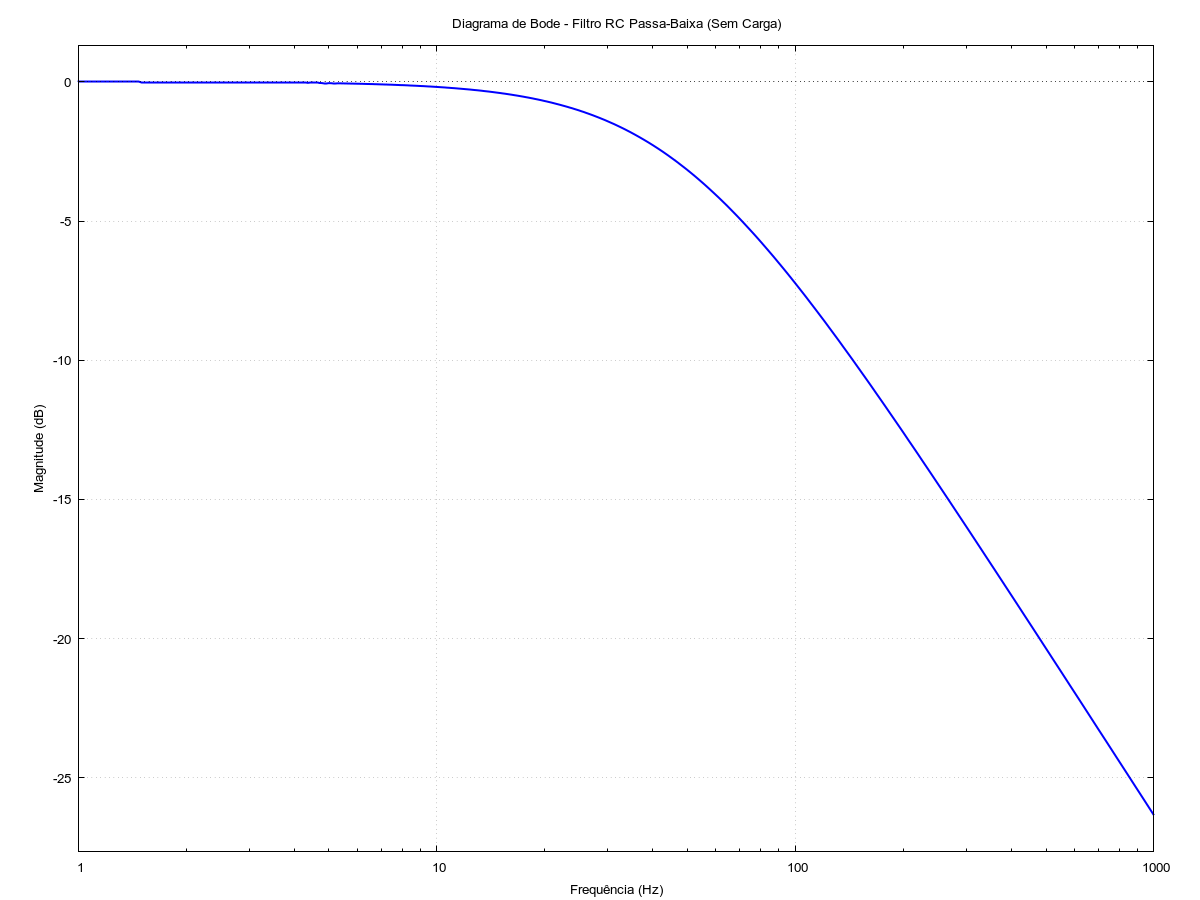
\includegraphics[width=0.7\textwidth]{FIGURAS/bode_teorico_circuito_1.png}
	\caption{Diagrama de Bode de magnitude teórico recalculado para $R = 33\text{ k}\Omega$ (Circuito 1).}
	\label{fig:bode_c1}
\end{figure}

\section{Circuito 2: Filtro RC Acoplado à Carga}

No segundo circuito, uma resistência de carga $R_L = 22\text{ k}\Omega$ é conectada em paralelo com o capacitor do filtro.

\begin{figure}[H]
	\centering
	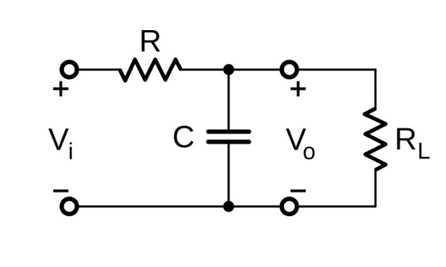
\includegraphics[width=0.6\textwidth]{FIGURAS/esquematico_circuito_2.png}
	\caption{Esquemático do filtro RC sujeito à carga resistiva $R_L$ (Circuito 2).}
	\label{fig:esquematico_c2}
\end{figure}

A impedância vista na saída passa a ser o paralelo entre o capacitor e a carga: $Z_p = \frac{R_L \cdot \frac{1}{sC}}{R_L + \frac{1}{sC}}$. Substituindo este novo bloco equivalente no divisor de tensão, a função de transferência modifica-se para:

\begin{equation}
	H_2(s) = \frac{Z_p}{R + Z_p}
\end{equation}

Através da rotina de simplificação de racionais do Maxima (\texttt{ratsimp}), a função resultante é expressa por:

\begin{equation}
	H_2(s) = \frac{R_L}{s \cdot C \cdot R \cdot R_L + R + R_L}
	\label{eq:h2}
\end{equation}

\subsection{Dedução Algébrica (Rascunhos)}

Os cálculos manuscritos detalhando a impedância equivalente $Z_p$ e a expansão algébrica do denominador estão expostos nas Figuras \ref{fig:rascunho_c2_1} e \ref{fig:rascunho_c2_2}.

\begin{figure}[H]
	\centering
	\begin{minipage}{0.45\textwidth}
		\centering
		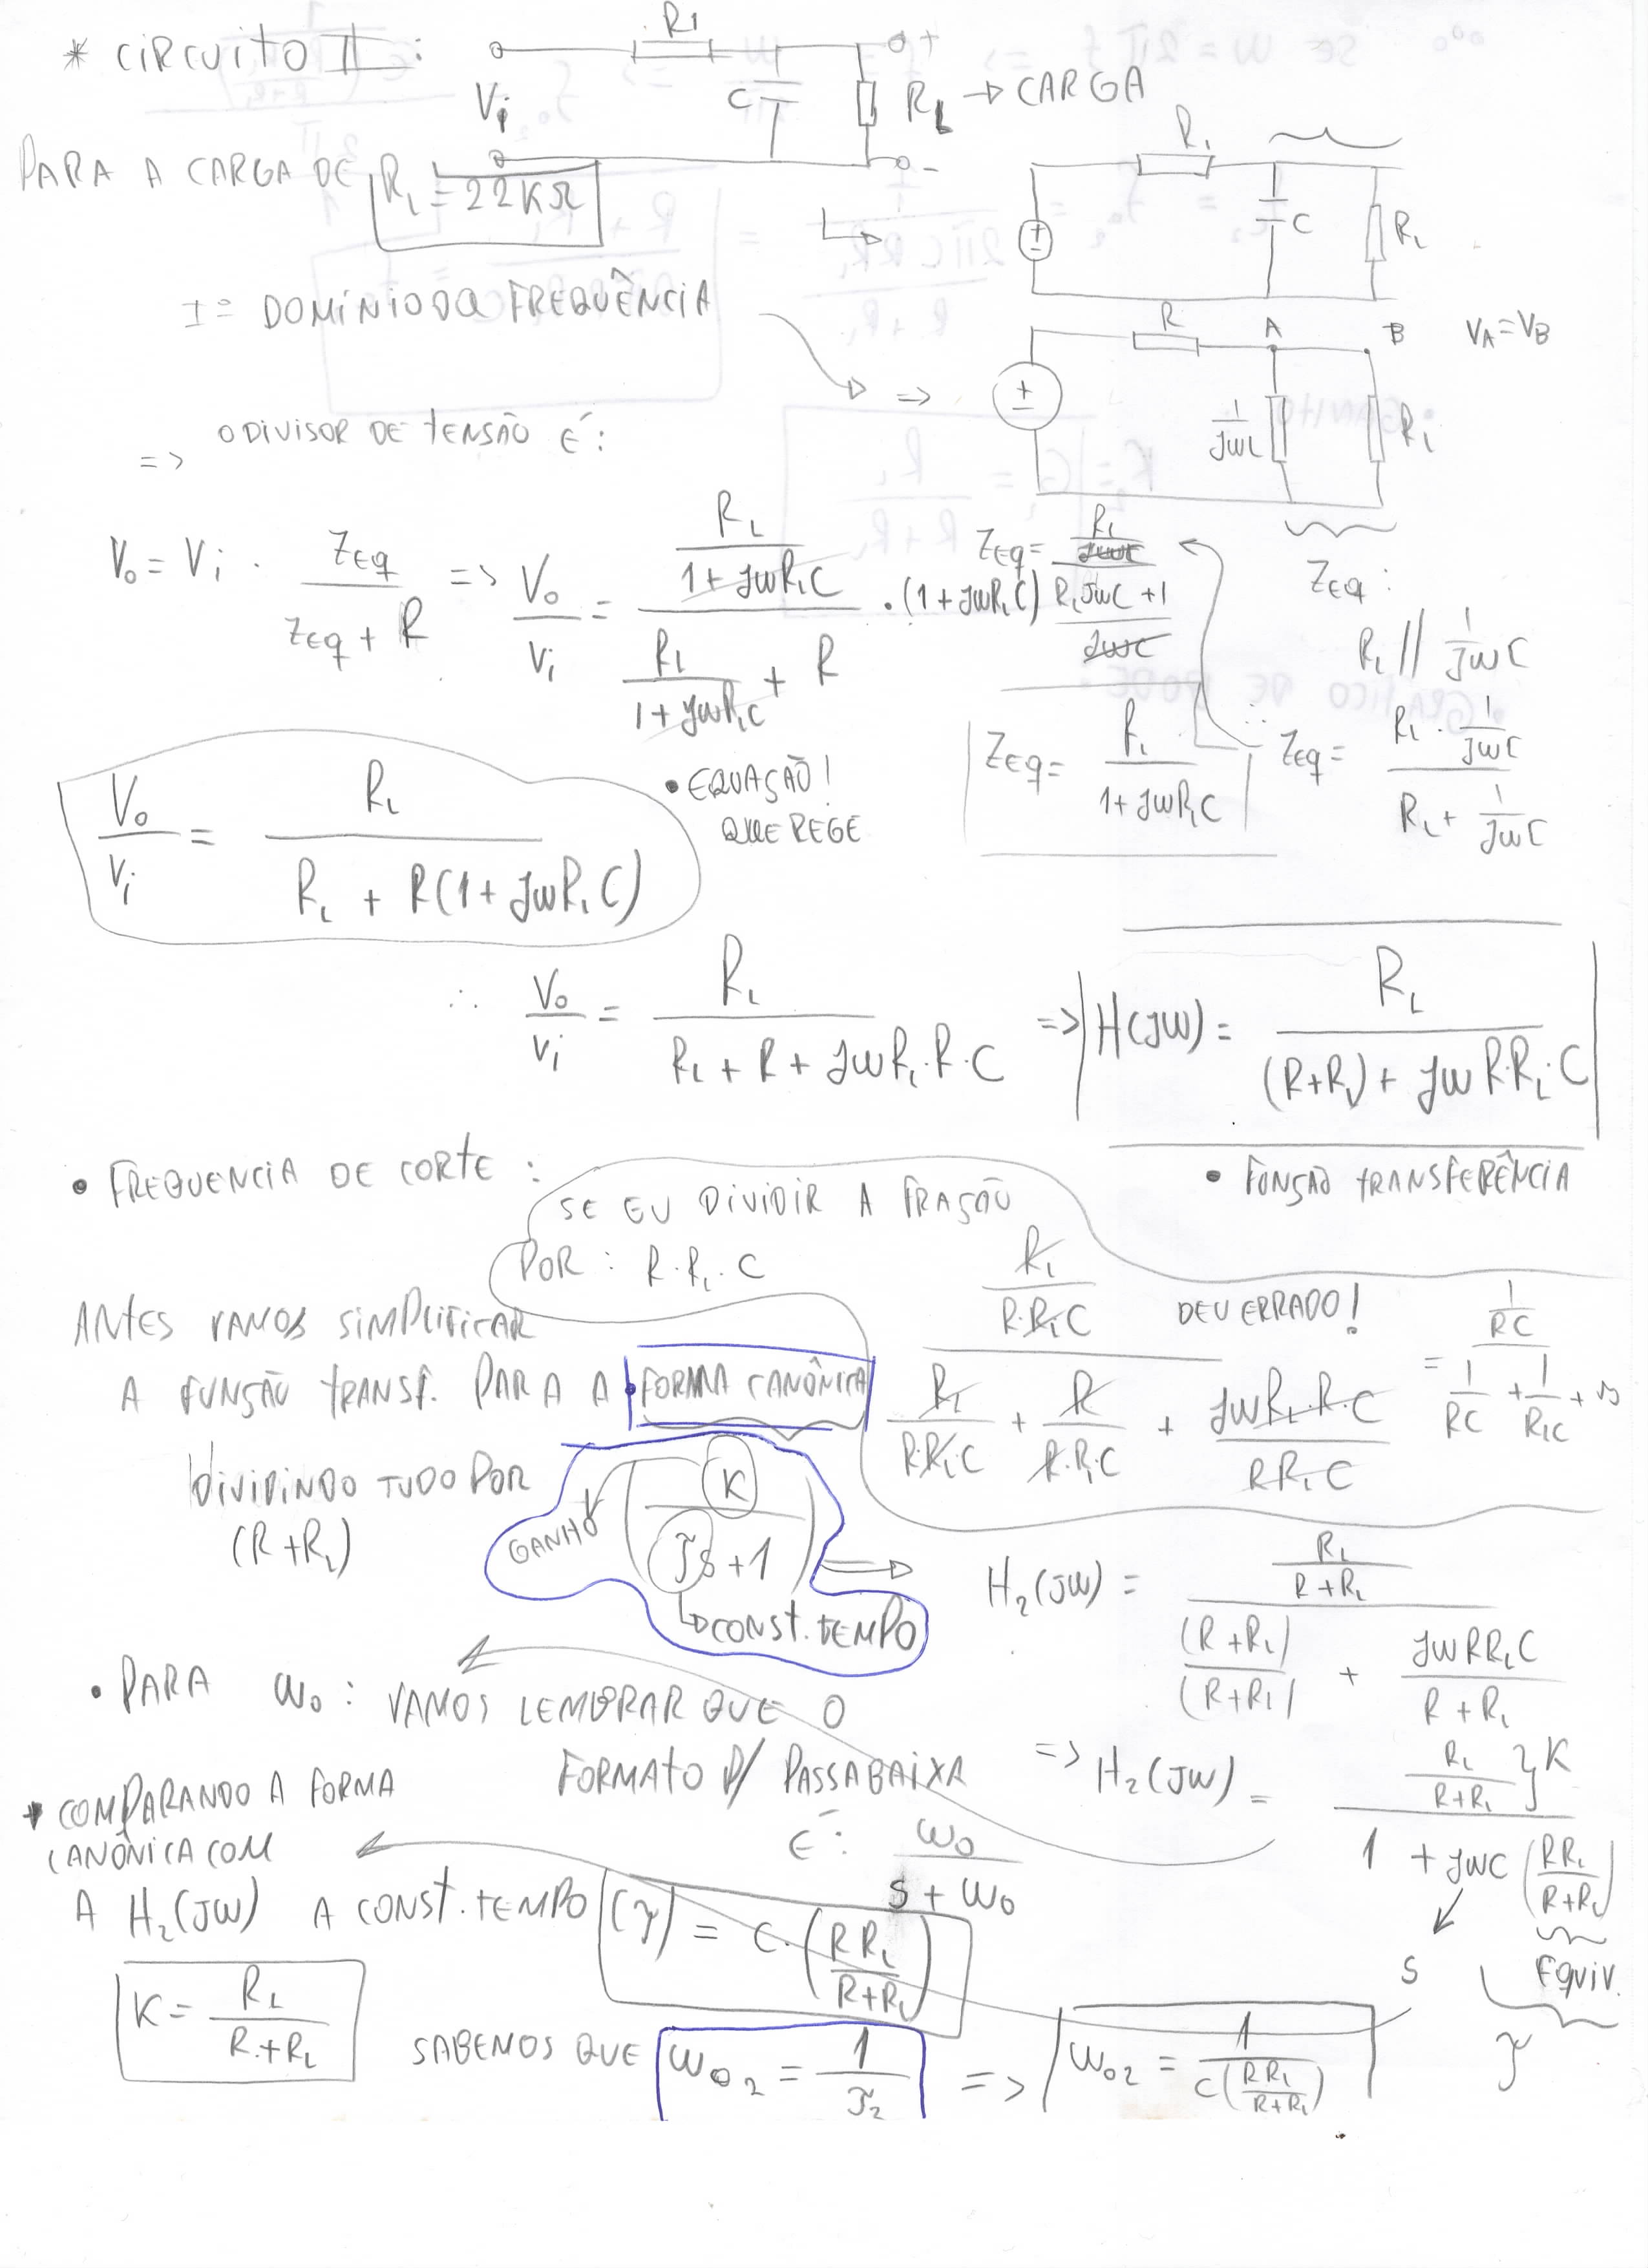
\includegraphics[width=\textwidth]{FIGURAS/rascunho_circuito_2_1.png}
		\caption{Associação em paralelo de $R_L$ e $C$.}
		\label{fig:rascunho_c2_1}
	\end{minipage}\hfill
	\begin{minipage}{0.45\textwidth}
		\centering
		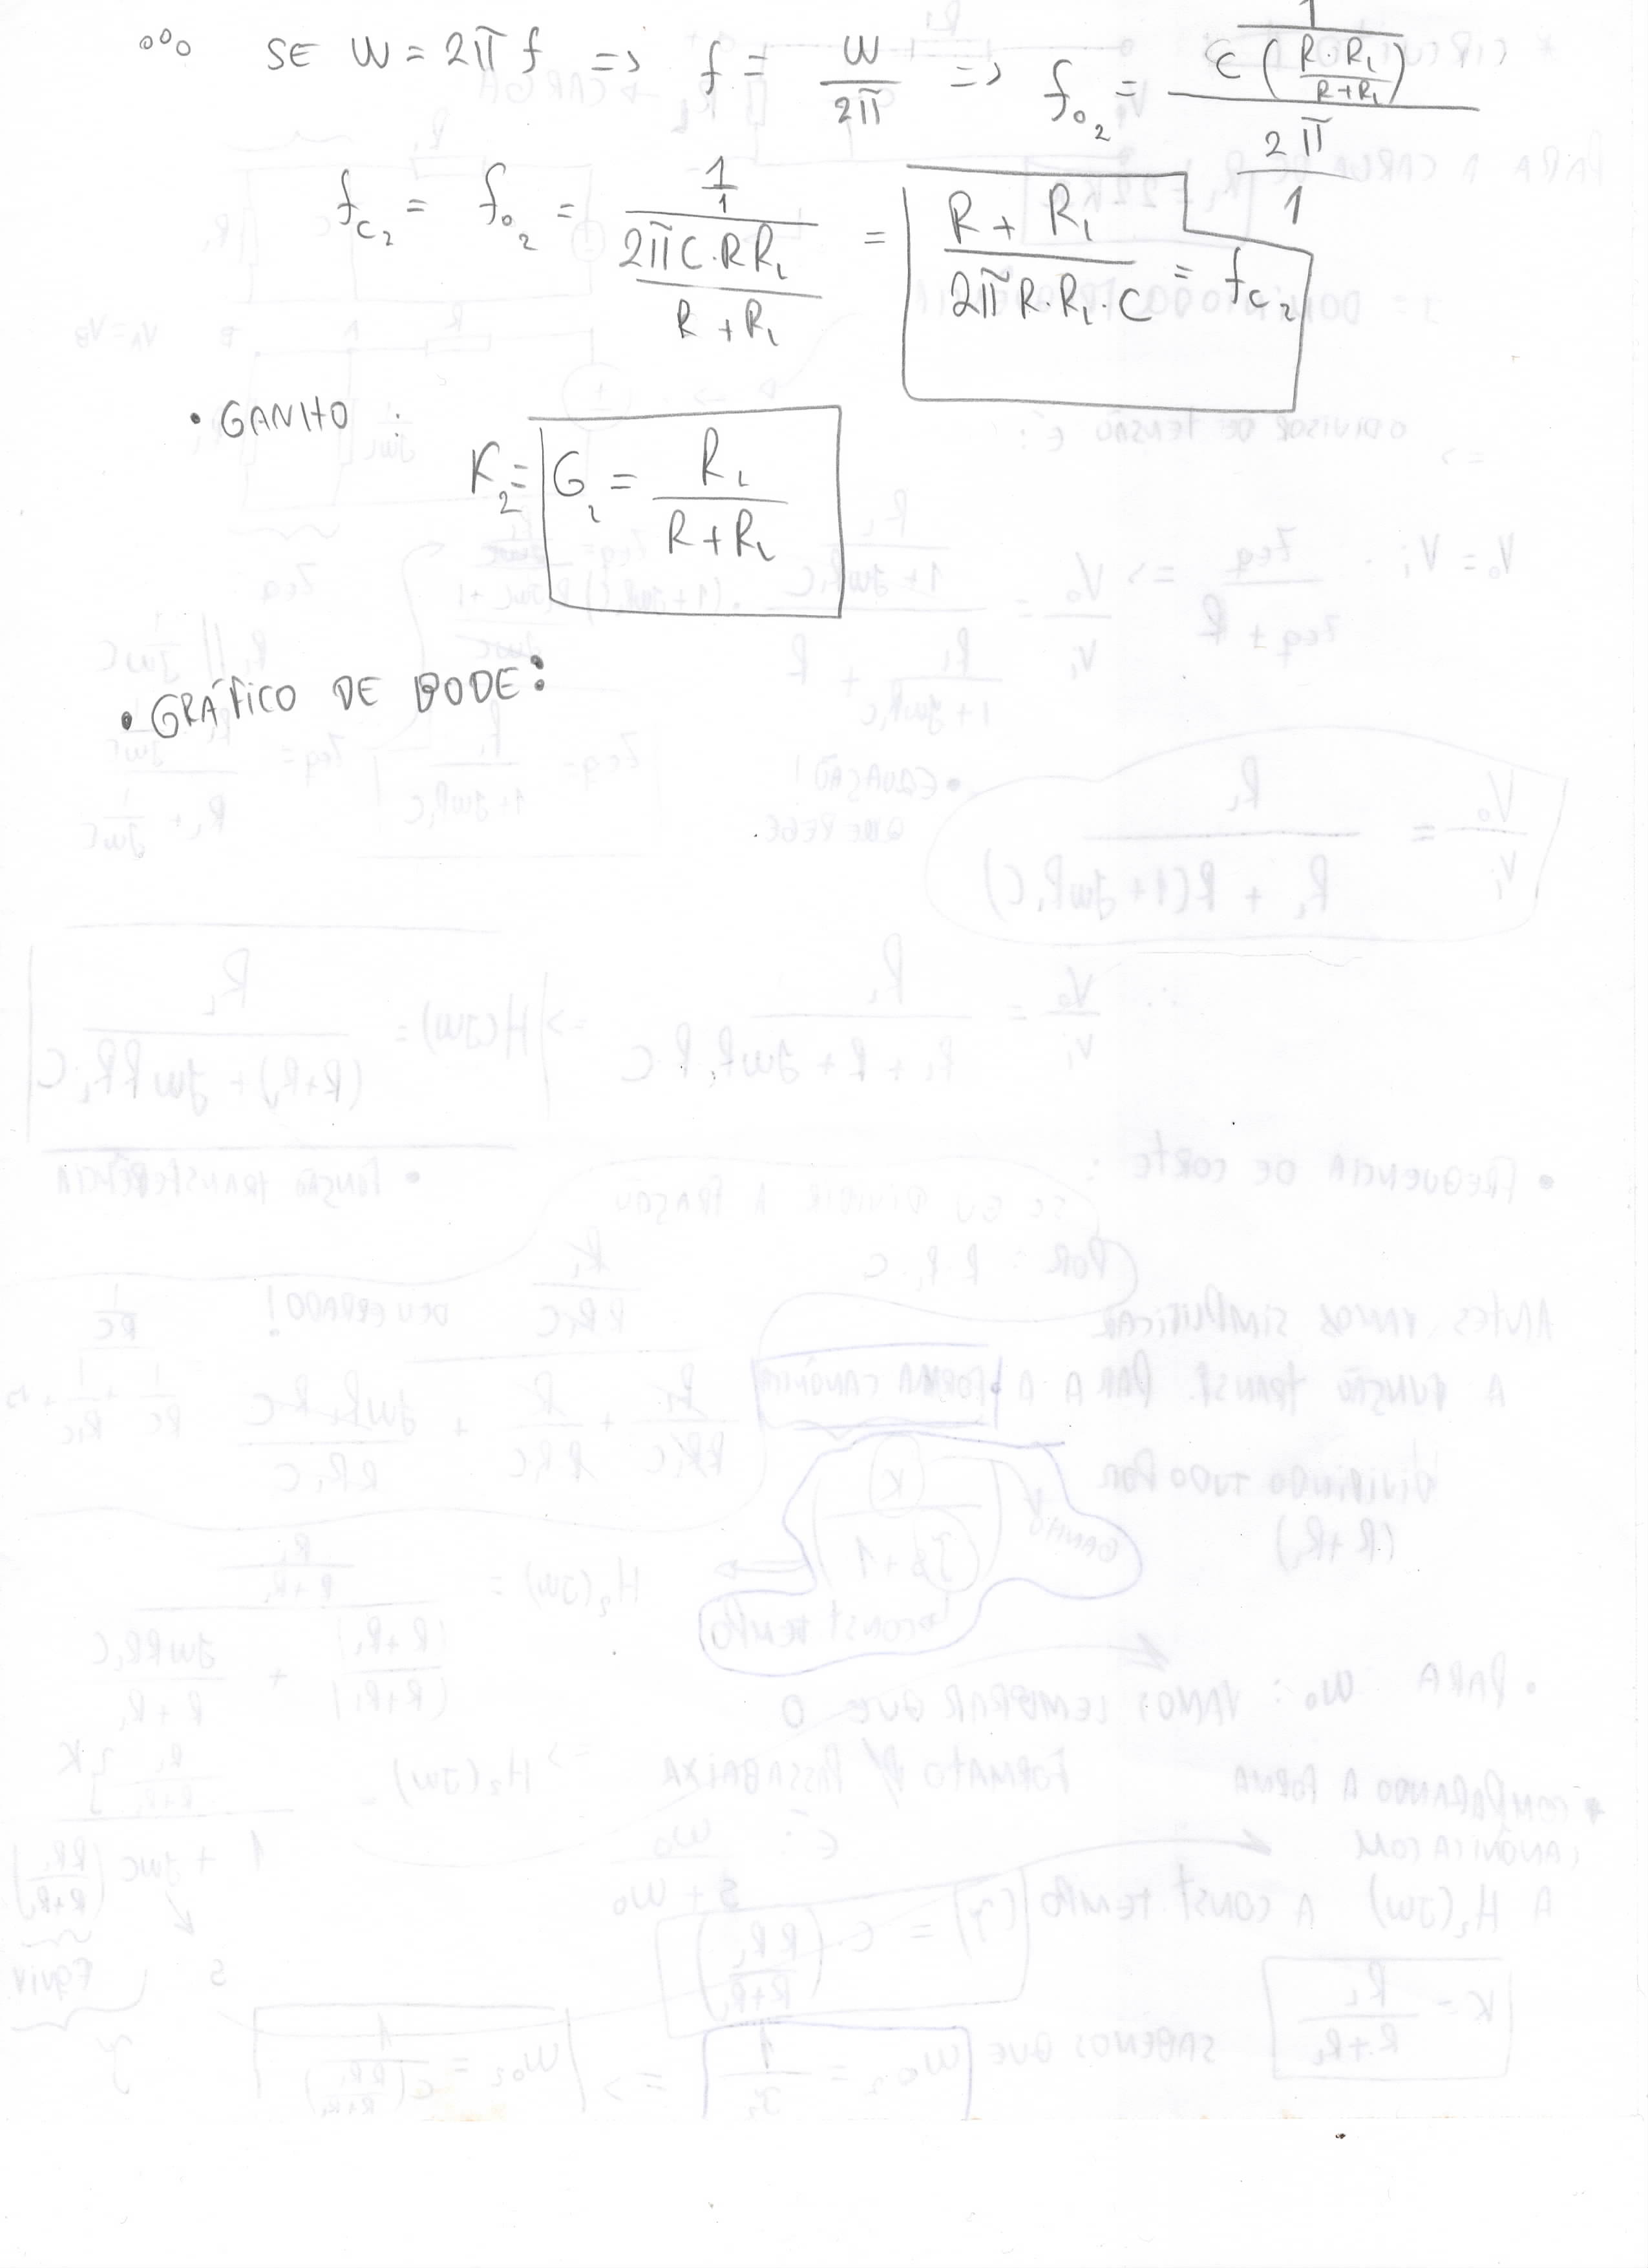
\includegraphics[width=\textwidth]{FIGURAS/rascunho_circuito_2_2.png} 
		\caption{Dedução completa de $H_2(s)$.}
		\label{fig:rascunho_c2_2}
	\end{minipage}
\end{figure}

\subsection{O Efeito de Carga: Atenuação e Desvio de Frequência}

A introdução de $R_L$ degrada substancialmente o desempenho do filtro. O ganho DC (para $s \to 0$) deixa de ser unitário, caindo para a relação restritamente resistiva:

\begin{equation}
	A_v = \frac{R_L}{R + R_L} = \frac{22\text{k}}{33\text{k} + 22\text{k}} = 0,405\text{ V/V } (\approx -7,8\text{ dB})
\end{equation}

Além da atenuação drástica na banda de passagem, a resistência equivalente percebida pelo capacitor no momento da descarga é agora o paralelo entre a resistência do filtro e a carga ($R_{eq} = R \parallel R_L$). Isso desloca severamente a frequência de corte para a direita do espectro:

\begin{equation}
	f_{c2} = \frac{R + R_L}{2\pi \cdot R \cdot R_L \cdot C} = \frac{33\text{k} + 22\text{k}}{2\pi \cdot 33\text{k} \cdot 22\text{k} \cdot 100\text{n}} \approx 121,6\text{ Hz}
\end{equation}

O diagrama de Bode teórico da Figura \ref{fig:bode_c2} evidencia este problema clássico: o sinal já inicia atenuado em baixa frequência e a banda de rejeição ocorre muito depois dos $50\text{ Hz}$ projetados originais.

\begin{figure}[H]
	\centering
	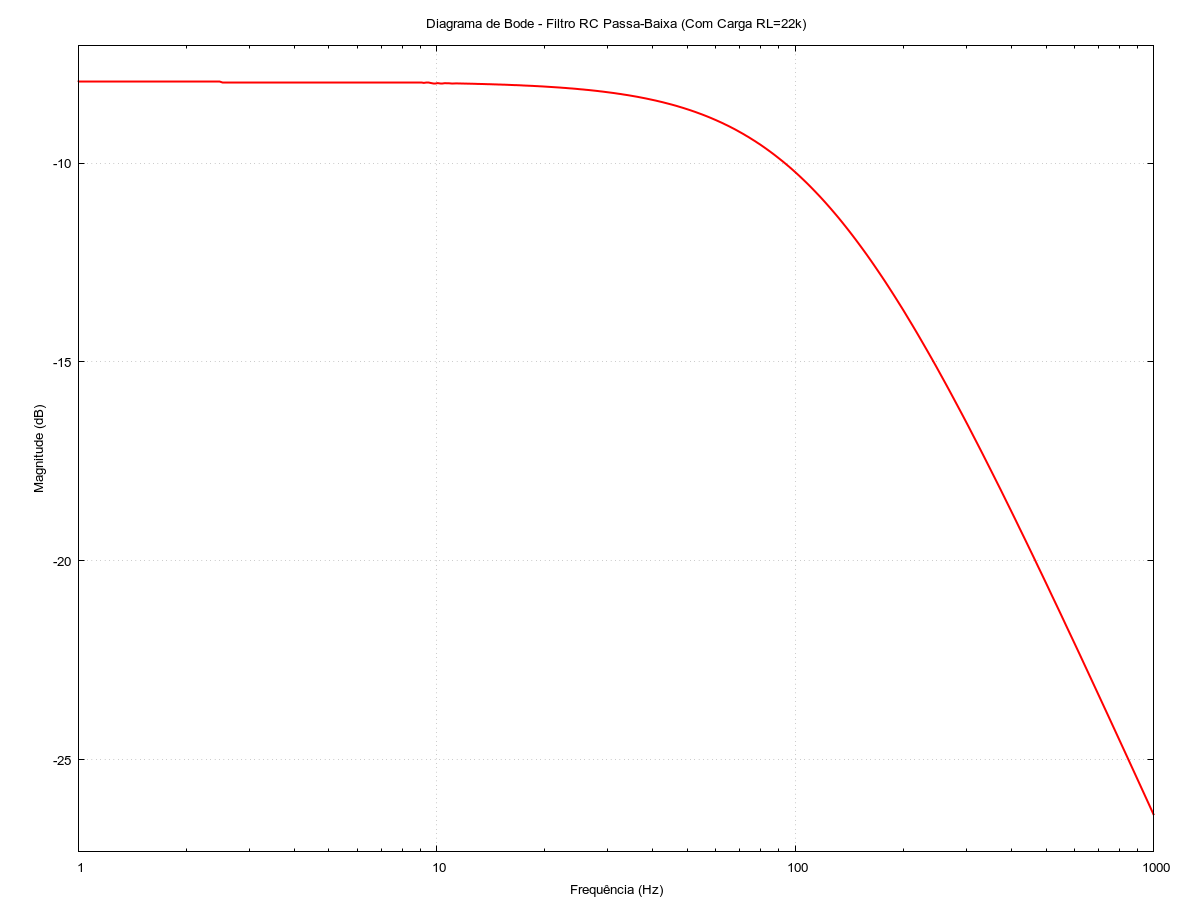
\includegraphics[width=0.7\textwidth]{FIGURAS/bode_teorico_circuito_2.png}
	\caption{Diagrama de Bode de magnitude evidenciando o Efeito de Carga no Circuito 2.}
	\label{fig:bode_c2}
\end{figure}

\section{Circuito 3: Isolamento Ativo com \textit{Buffer}}

Para neutralizar o efeito de carga observado no Circuito 2, interpôs-se um amplificador operacional na configuração não-inversora de ganho unitário (\textit{buffer}) entre o estágio passivo RC e a carga $R_L$.

\begin{figure}[H]
	\centering
	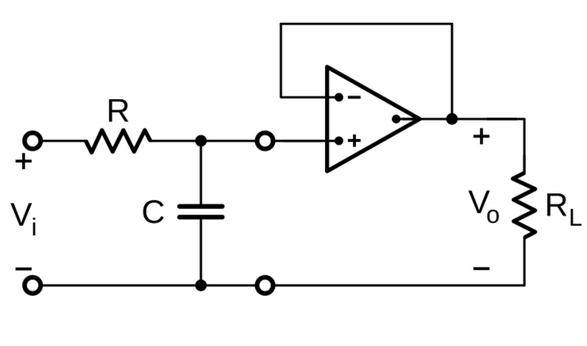
\includegraphics[width=0.6\textwidth]{FIGURAS/esquematico_circuito_3.png}
	\caption{Esquemático do filtro RC isolado da carga por um \textit{buffer} ativo (Circuito 3).}
	\label{fig:esquematico_c3}
\end{figure}

\subsection{Dedução Algébrica e Restauração da Dinâmica}

De acordo com o modelo ideal do amplificador operacional, os seus terminais de entrada possuem impedância infinita ($i_{in} = 0$). Consequentemente, o nó de tensão da entrada não-inversora ($V^+$) não drena qualquer corrente do divisor RC. Assim, a tensão $V^+$ é rigorosamente idêntica à saída do Circuito 1 em vazio.

O diagrama manuscrito da Figura \ref{fig:rascunho_c3_1} formaliza a modelagem das correntes nodais nulas e o curtocircuito virtual da malha de realimentação negativa ($V^- = V^+$), provando que a tensão na carga $V_o$ acopla perfeitamente a tensão originada pelo filtro capacitivo.

\begin{figure}[H]
	\centering
	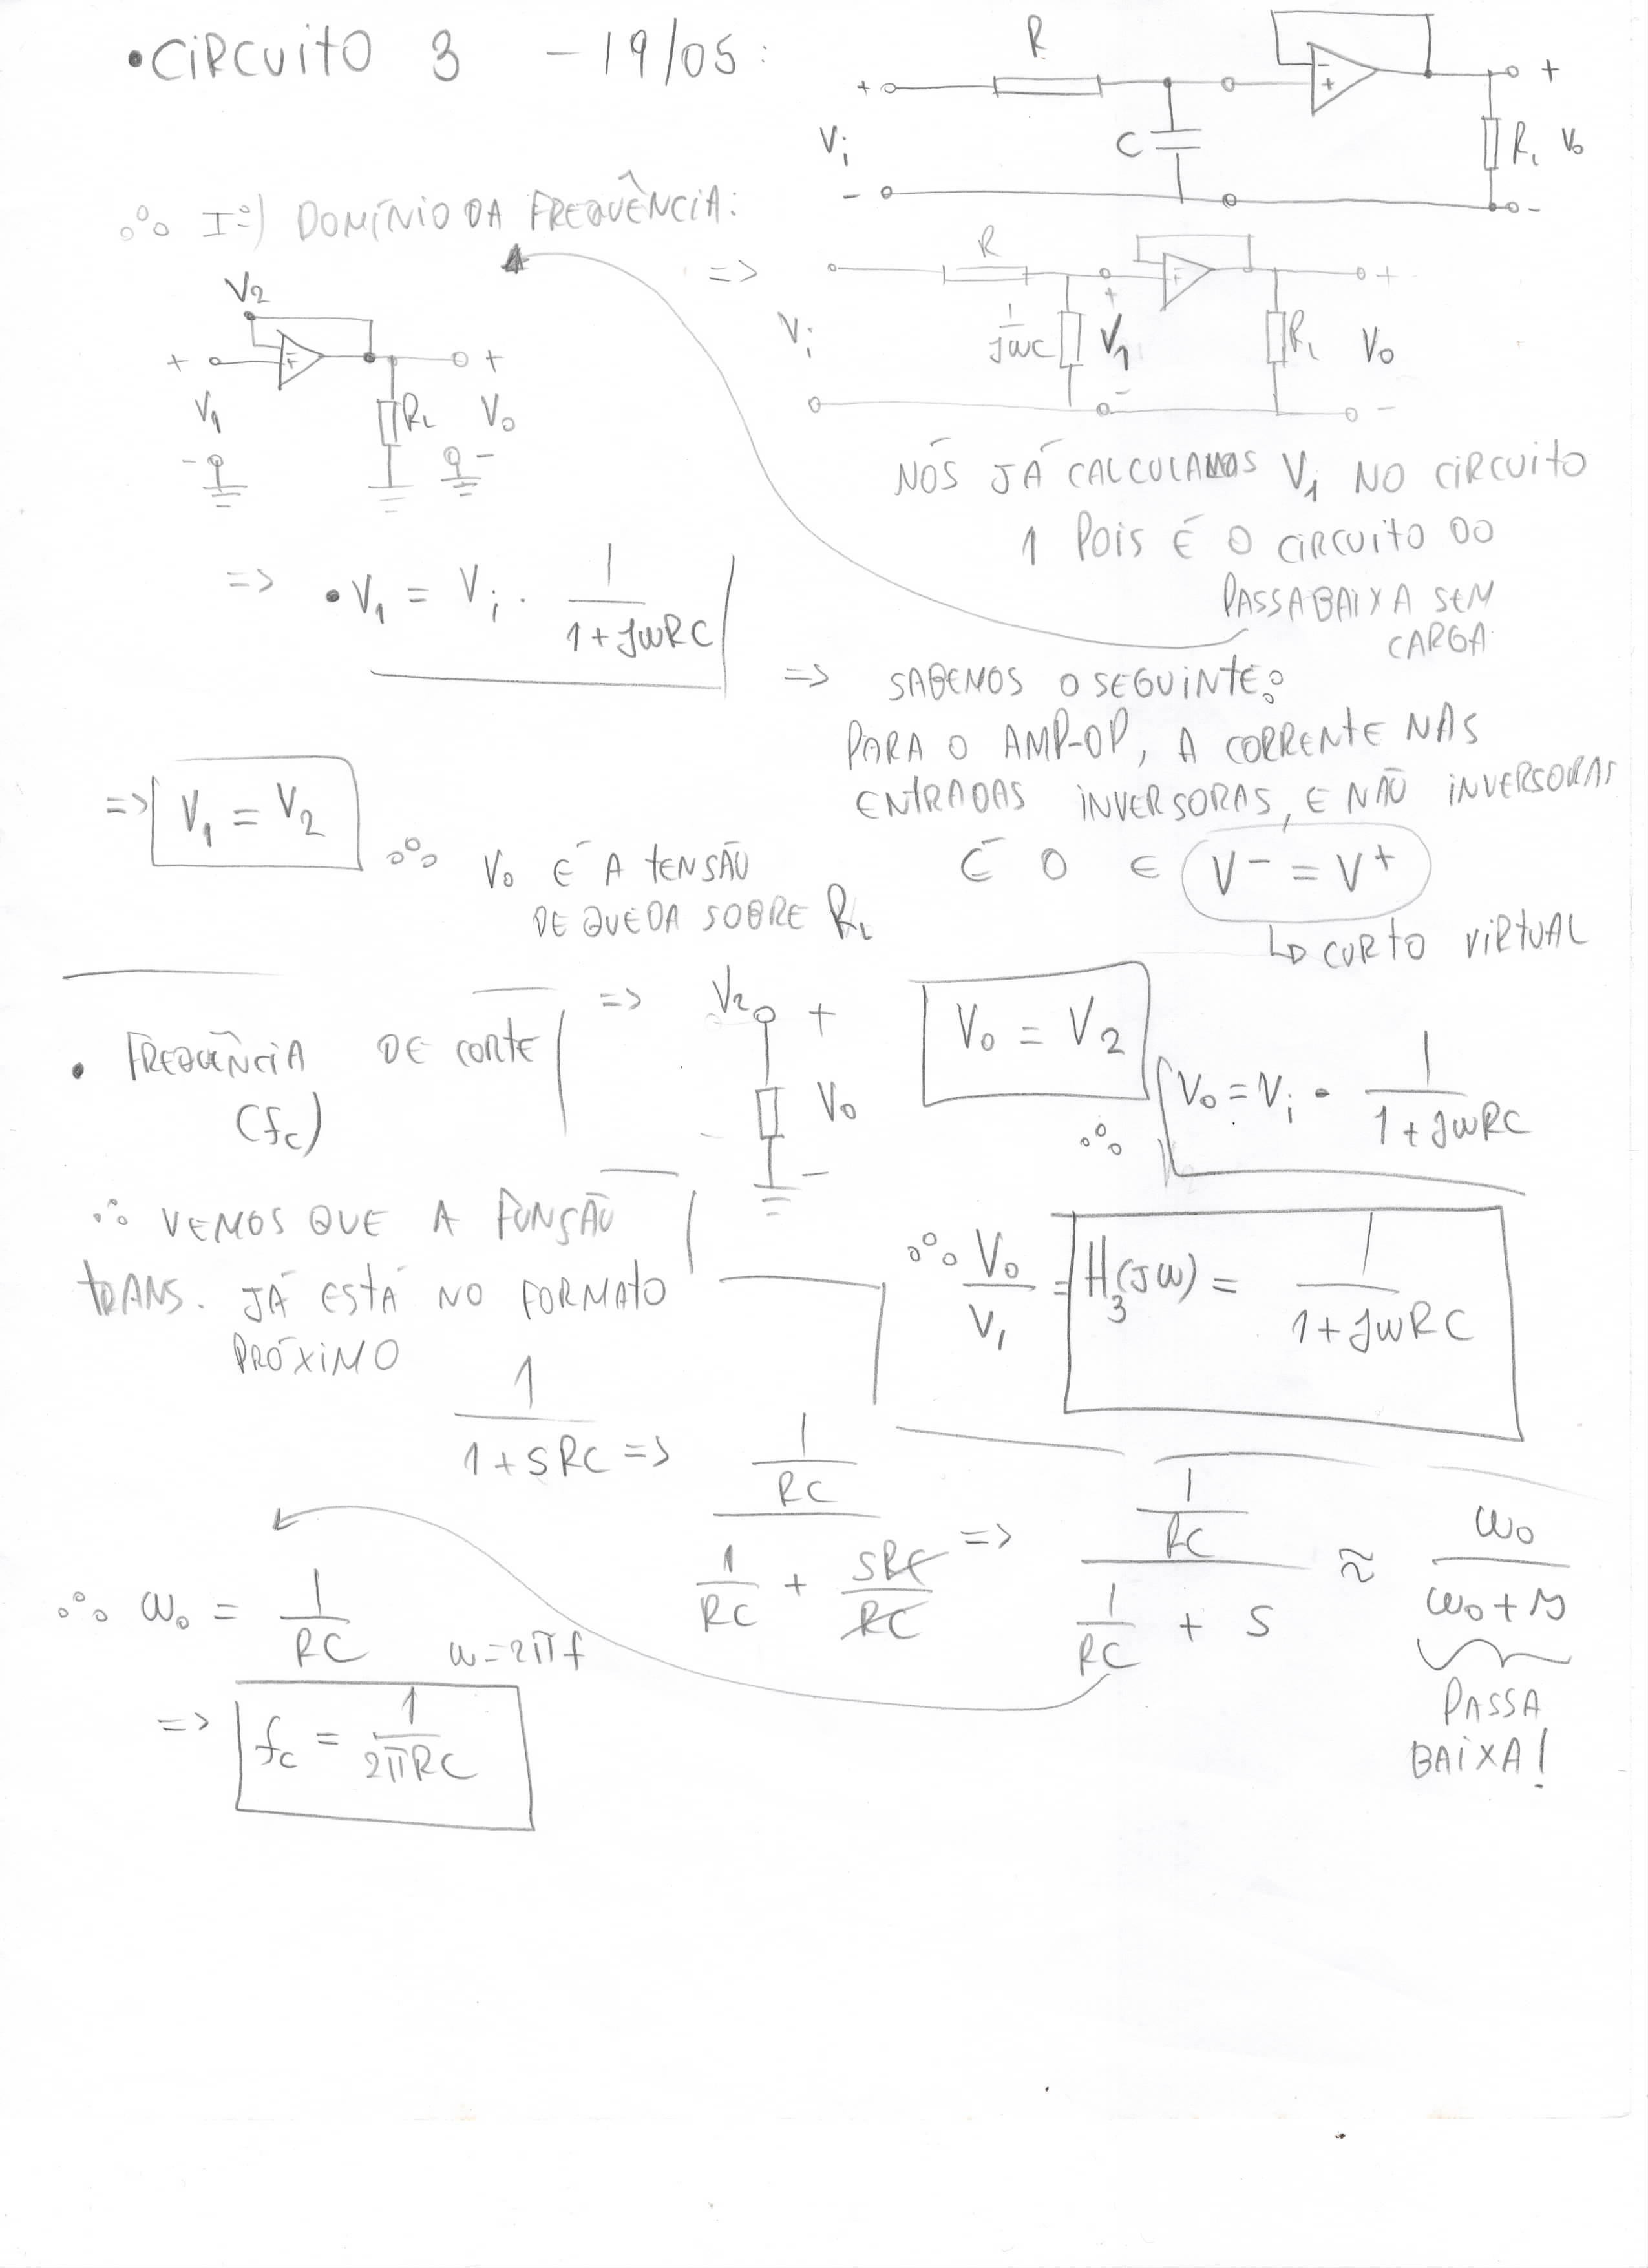
\includegraphics[width=0.5\textwidth]{FIGURAS/rascunho_circuito_3_1.png}
	\caption{Análise nodal do \textit{buffer} evidenciando a impedância de entrada infinita.}
	\label{fig:rascunho_c3_1}
\end{figure}

Desta forma, a função de transferência global $H_3(s)$ retorna à forma pura isolada da Equação \ref{eq:h1}:

\begin{equation}
	H_3(s) = \frac{1}{RCs + 1}
\end{equation}

Ao rodar os parâmetros reais do laboratório ($R = 33\text{ k}\Omega$, $C = 100\text{ nF}$, $R_L = 22\text{ k}\Omega$) no Maxima, a matemática prova que o valor de $R_L$ é eliminado do denominador paramétrico. O ganho de tensão retorna a $1\text{ V/V}$ ($0\text{ dB}$) e a frequência de corte restaura-se para os seus originários $\approx 48,23\text{ Hz}$.

\begin{figure}[H]
	\centering
	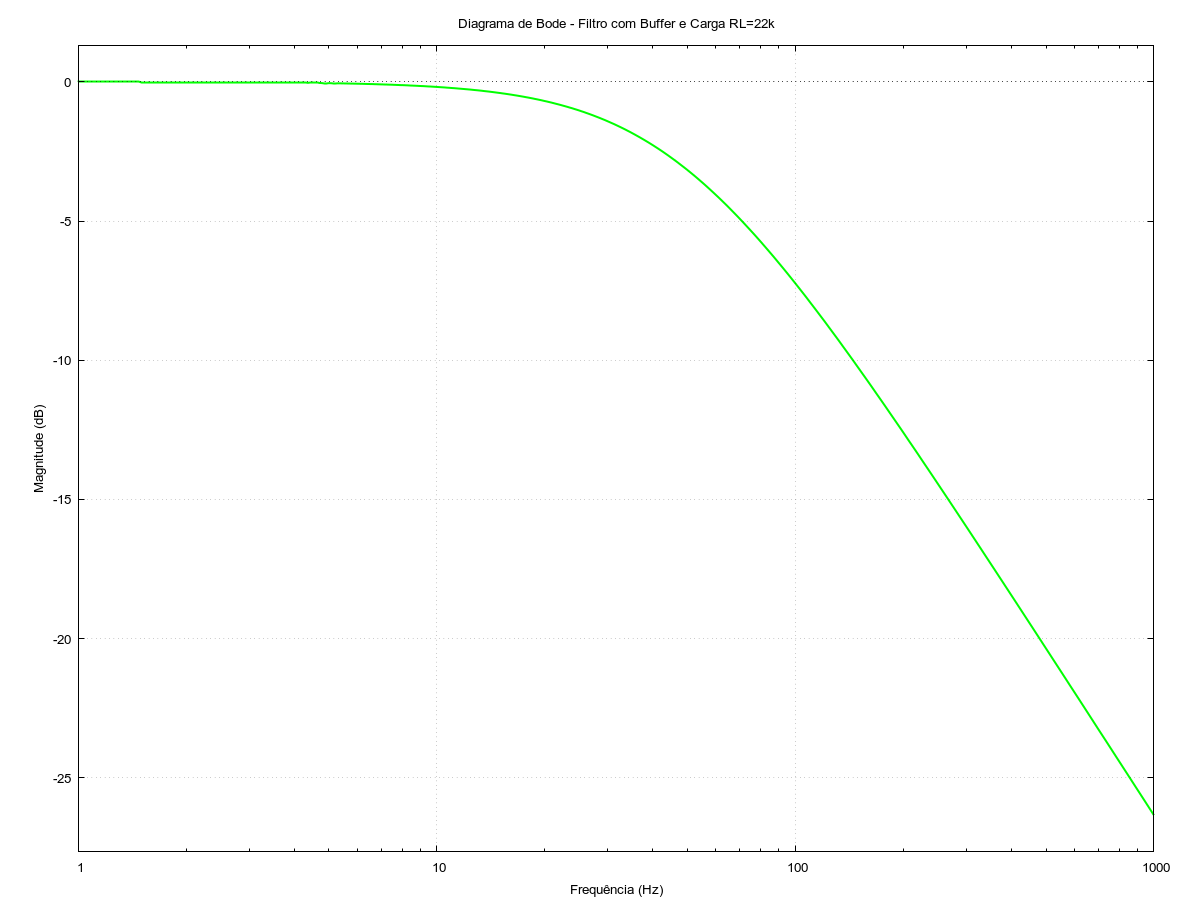
\includegraphics[width=0.7\textwidth]{FIGURAS/bode_teorico_circuito_3.png}
	\caption{Diagrama de Bode teórico do Circuito 3. A curva coincide perfeitamente com o projeto inicial do Circuito 1.}
	\label{fig:bode_c3}
\end{figure}